\documentclass[alsotrans]{beamerswitch}
\usepackage{fprog}

\title[Среди и процеси]{Модел на средите и изчислителни процеси}

\date{13 октомври 2021 г.}

\lstset{language=Scheme}

\begin{document}

\begin{frame}
  \titlepage
\end{frame}

\section{Модел на средите}

\begin{frame}
  \frametitle{Среди в Scheme}

  \begin{itemize}[<+->]
  \item Връзката между символите и техните оценки се записват в речник, който се нарича \textbf{среда}.
  \item Всеки символ има най-много една оценка в дадена среда.
  \item В даден момент могат да съществуват много среди.
  \item Символите винаги се оценяват в една конкретна среда.
  \item \alert{Символите могат да има различни оценки в различни среди.}
  \item При стартиране Scheme по подразбиране работи в \textbf{глобалната среда}.
  \item В глобалната среда са дефинирани символи за стандартни операции и функции.
  \end{itemize}
\end{frame}

\begin{frame}
  \frametitle{Пример за среда}

  \begin{columns}[T,onlytextwidth]
    \begin{column}{.5\textwidth}
      \begin{itemize}[<+->]
      \item \lst{(define a 8)}
      \item \evalstoerr r
      \item \lst{(define r 5)}
      \item \evalsto{(+ r 3)}8
      \item \lst{(define (f x) (* x r))}
      \item \evalsto{(f 3)}{15}
      \item \evalsto{(f r)}{25}
      \end{itemize}
    \end{column}

    \begin{column}{.5\textwidth}
      \begin{tikzpicture}
        \envir{E}{
          \kv a8
          \only<3->{\kv r5}
          \only<5->{\kf fx{(* x r)}E}
        }
      \end{tikzpicture}
    \end{column}
  \end{columns}
\end{frame}

\begin{frame}
  \frametitle{Функции и среди}

  \begin{itemize}[<+->]
  \item Всяка функция \tt f пази указател към средата \env E, в която е дефинирана.
  \item При извикване на \tt f:
    \begin{itemize}
    \item създава се нова среда \env{E_1}, която разширява \env E
    \item в \env{E_1} всеки символ означаващ формален параметър се свързва с оценката на фактическия параметър
    \item тялото на $f$ се оценява в \env{E_1}
    \end{itemize}
  \end{itemize}
\end{frame}

\begin{frame}
  \frametitle{Дърво от среди}
  \begin{itemize}[<+->]
  \item Всяка среда пази указател към своя ``родителска среда'', която разширява
  \item така се получава дърво от среди
  \item при оценка на символ в дадена среда \env E
    \begin{itemize}
    \item първо се търси оценката му в \env E
    \item ако символът не е дефиниран в \env E, се преминава към родителската среда
    \item при достигане на най-горната среда, ако символът не е дефиниран и в нея се извежда съобщение за грешка
    \end{itemize}
  \end{itemize}
\end{frame}

\begin{frame}
  \frametitle{Извикване на дефинирана функция}

  \begin{fixedarea}
    \begin{columns}[T,onlytextwidth]
      \begin{column}{.5\textwidth}
        \begin{itemize}[<+->]
        \item \lst{(define r 5)}
        \item \lst{(define a 3)}
        \item \lst{(define (f x) (* x r))}\\[2ex]
          \evalchain{
            "(f a)"[env=E] ->
            "(f 3)"[env=E] ->
            "(* x r)"[env=E_1] ->
            "15";
          }
        \end{itemize}
      \end{column}

      \begin{column}{.5\textwidth}
        \begin{tikzpicture}
          \envir{E}{
            \kv r5
            \only<2->{\kv a3}
            \only<3->{\kf fx{(* x r)}E}
          }
          \childenvir[6-]{below=5em}E{E_1}{\kv x3}
        \end{tikzpicture}
      \end{column}
    \end{columns}
  \end{fixedarea}
\end{frame}

\section{Рекурсия}

\subsection{Рекурсивни функции}

\begin{frame}
  \frametitle{Какво е рекурсия?}

  \pause
  \begin{center}
    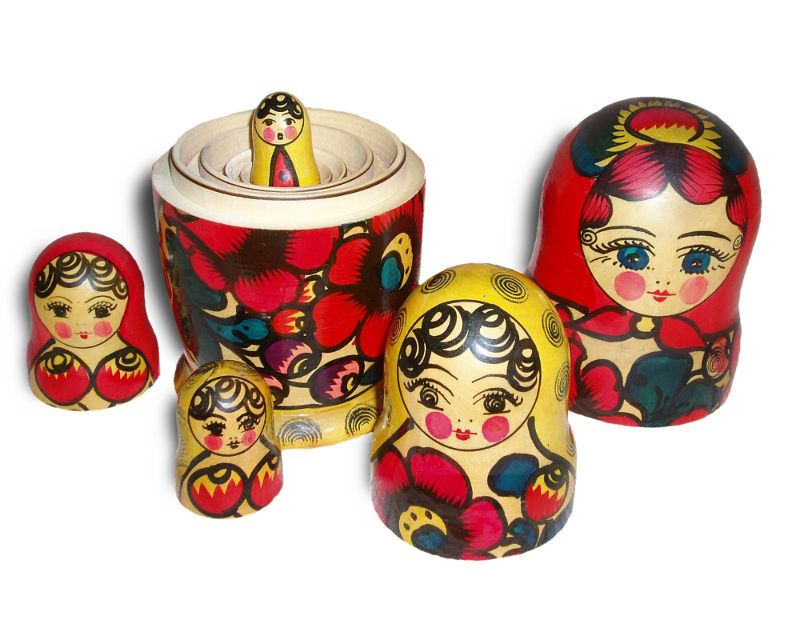
\includegraphics[width=0.7\textwidth]{images/matroska.jpg}\\
    \imageAttr{Matryoshka dolls}{User:Fanghong (оригинал) и User:Gnomz007 (производна)}{https://commons.wikimedia.org/wiki/File:Russian-Matroshka_no_bg.jpg}{CC BY-SA 3.0}
  \end{center}
\end{frame}

\begin{frame}
  \frametitle{Какво е рекурсия?}

  \begin{center}
    % TODO: да се нарисува с TikZ и foreach
    
\includegraphics[width=0.9\textwidth]{images/sierpinski.png}
  \end{center}
\end{frame}

\begin{frame}
  \frametitle{Какво е рекурсия?}

  \pause
  Повторение чрез позоваване на себе си\\[2ex]
  \pause
  Рекурсивна функция: дефинира се чрез себе си\\
  \begin{equation*}
    n! = \left\{
    \begin{array}{l@{}l@{\qquad}l}
      1,&\text{ при }n = 0,&\textbf{(база)}\\
      n\cdot (n-1)!,&\text{ при }n > 0.&\textbf{(стъпка)}
    \end{array}\right.
  \end{equation*}\\[2ex]
  \pause
  \begin{itemize}
  \item Дава се отговор на най-простата задача (база, дъно)
  \item Показва се как сложна задача се свежда към една или няколко по-прости задачи от същия вид (стъпка)
  \end{itemize}
\end{frame}


\begin{frame}
  \frametitle{Рекурсивни уравнения}

  Какво означава ``да дефинираме функция чрез себе си''?\\[2ex]
  \pause
  Да разгледаме \emph{рекурсивното уравнение}, в което $F$ е неизвестно:
  \begin{equation*}
    F(n) =
    \underbrace{\begin{cases}
      1,&\text{ при }n = 0,\\
      n \cdot F(n-1),&\text{ при }n > 0.
    \end{cases}}_{\Gamma(F)(n)}
  \end{equation*}
  \pause
  \alert{$n!$ е ``най-малкото'' решение на уравнението $F = \Gamma(F)$.}
\end{frame}

\begin{frame}[fragile]
  \frametitle{Най-малка неподвижна точка}

  \begin{theorem}[Knaster-Tarski]
    Ако $\Gamma$ е изчислим оператор, то уравнението $F = \Gamma(F)$ има единствено най-малко решение $f$ \pause (\textbf{най-малка неподвижна точка на $\Gamma$}). \pause Нещо повече, решението точно съответства на рекурсивна програма пресмятаща $f$ чрез $\Gamma$.
  \end{theorem}
  \pause
\begin{lstlisting}
(define (fact n)
  (if (= n 0) 1
      (* n (fact (- n 1)))))
\end{lstlisting}
  \pause
  Кое е \textbf{най-малкото решение} на уравнението $F(x) = F(x+1) - 1$?
  \pause
\lstinline{(define (g x) (- 1 (g (+ x 1)))}\\
\evalsto{(f 0)}?\\
  \pause
  $g$ е ``празната функция'', т.е. $\mathrm{dom}(g) = \emptyset$.
\end{frame}

\begin{frame}
  \frametitle{Операционна и денотационна семантика}

  Два подхода за описание на смисъла на функциите в Scheme.\\
  \pause
  Нека \tt{(define (f x) $\Gamma$[f])} е рекурсивно дефинирана функция.\\
  \pause
  \alert{Коя е математическата функция $f$, която се пресмята от \tt f?}\\[2ex]
  \pause
  \textbf{Денотационна семантика}\\
  $f$ е най-малката неподвижна точка на уравнението $F = \Gamma(F)$.\\[2ex]
  \pause
  \textbf{Операционна семантика}\\
  Разглеждаме редицата от последователни оценки на комбинации\\
  \tt{(f a)} $\rightarrow$ \tt{$\Gamma$[f][x $\mapsto$ a]} $\rightarrow\ldots$\\
  Ако стигнем до елемент \tt b, който не е комбинация, то $f(a) := b$.\\[2ex]
  \pause
  \alert{Функциите в Scheme имат дуален, но еквивалентен смисъл:}
  \begin{itemize}
  \item решения на рекурсивни уравнения
  \item изчислителни процеси, генериращи се при оценка
  \end{itemize}
\end{frame}

\subsection{Рекурсивни процеси}

\begin{frame}
  \frametitle{Оценка на рекурсивна функция}

  \begin{center}
    \sizeboth\scriptsize
    % TODO: да се реализира с foreach
    \evalchain[(-1)]{
      "\lst{(fact 4)}" ->
      "\alt<+->{\lst{(* 4 (fact 3))}}
      {\lst{(if (= 4 0) 1 (* 4 (fact (- 4 1))))}}" ->
      "\alt<+->{\lst{(* 4 (* 3 (fact 2)))}}
      {\lst{(* 4 (if (= 3 0) 1 (* 3 (fact (- 3 1)))))}}" ->
      "\alt<+->{\lst{(* 4 (* 3 (* 2 (fact 1))))}}
      {\lst{(* 4 (* 3 (if (= 2 0) 1 (* 2 (fact (- 2 1))))))}}" ->
      "\alt<+->{\lst{(* 4 (* 3 (* 2 (* 1 (fact 0)))))}}
      {\lst{(* 4 (* 3 (* 2 (if (= 1 0) 1 (* 1 (fact (- 1 1)))))))}}" ->
      "\alt<+->{\lst{(* 4 (* 3 (* 2 (* 1 1))))}}
      {\lst{(* 4 (* 3 (* 2 (* 1 (if (= 0 0) 1 (* 0 (fact (- 0 1))))))))}}" ->[v]
      "\lst{(* 4 (* 3 (* 2 1)))}" ->[v]
      "\lst{(* 4 (* 3 2))}" ->[v]
      "\lst{(* 4 6)}" ->[v]
      24;
    }
  \end{center}
\end{frame}

\begin{frame}
  \frametitle{Оценка на рекурсивна функция в среда}

  \begin{columns}[T,onlytextwidth]
    \sizeboth\tiny
    \begin{column}{.68\textwidth}
      \begin{center}
        % TODO: да се реализира с foreach
        \evalchain[(-1)]{
          "\lst{(fact 4)}"[env=E] ->
          "\alt<+->{\lst{(* 4 (fact 3))}}
          {\lst{(if (= n 0) 1 (* n (fact (- n 1))))}}"[env=E_1] ->
          "\alt<+->{\lst{(* 4 (* 3 (fact 2)))}}
          {\lst{(* 4 (if (= n 0) 1 (* n (fact (- n 1)))))}}"[env=E_2] ->
          "\alt<+->{\lst{(* 4 (* 3 (* 2 (fact 1))))}}
          {\lst{(* 4 (* 3 (if (= n 0) 1 (* n (fact (- n 1))))))}}"[env=E_3] ->
          "\alt<+->{\lst{(* 4 (* 3 (* 2 (* 1 (fact 0)))))}}
          {\lst{(* 4 (* 3 (* 2 (if (= n 0) 1 (* n (fact (- n 1)))))))}}"[env=E_4] ->
          "\alt<+->{\lst{(* 4 (* 3 (* 2 (* 1 1))))}}
          {\lst{(* 4 (* 3 (* 2 (* 1 (if (= n 0) 1 (* n (fact (- n 1))))))))}}"[env=\alt<10>{E_5}{E_4}] ->[v]
          "\lst{(* 4 (* 3 (* 2 1)))}"[envv=E_3] ->[v]
          "\lst{(* 4 (* 3 2))}"[envv=E_2] ->[v]
          "\lst{(* 4 6)}"[envv=E_1] ->[v]
          24[envv=E];
        }
      \end{center}
    \end{column}
    \begin{column}{.32\textwidth}
      \begin{tikzpicture}
        \envir{E}{\kf{fact}n\ldots E}
        \childenvir[2- ]{below left =2em and -2em}E{E_1}{\kv n4}
        \childenvir[4- ]{below      =2em         }E{E_2}{\kv n3}
        \childenvir[6- ]{below right=2em and -2em}E{E_3}{\kv n2}
        \childenvir[8- ]{below left =7em and -3em}E{E_4}{\kv n1}
        \childenvir[10-]{below right=7em and -3em}E{E_5}{\kv n0}
      \end{tikzpicture}
    \end{column}
  \end{columns}
  \vspace{2ex}
  \onslide<+->
  Линеен рекурсивен процес
\end{frame}

\subsection{Итеративни процеси}

\begin{frame}[fragile]
  \frametitle{Факториел с цикъл}

  \small
  \begin{columns}[T,onlytextwidth]
    \begin{column}{.5\textwidth}
      \textbf{Факториел на C++}\\
%TODO: може ли да се използва lstlisting тук?
\begin{semiverbatim}
\altbox<3| trans:0>{int fact(int n)} \{
  \altbox<4| trans:0>{int r = 1;}
  \altbox<0>{for(\altbox<5| trans:0>{int i = 1};\altbox<6| trans:0>{i <= n};\altbox<7>{i++})}
    \altbox<8| trans:0>{r *= i;}
  \altbox<9| trans:0>{return r;}
\}
\end{semiverbatim}
    \end{column}
    \pause
    \begin{column}{.5\textwidth}
      \textbf{Превод на Scheme}\\
%TODO: може ли да се използва lstlisting тук?
\begin{semiverbatim}
(define (for n \altbox<4,8| trans:0>{r}\altbox<5,7| trans:0>{i})
  (if \altbox<6| trans:0>{(<= i n)}
      (for n \altbox<8| trans:0>{(* r i)}\altbox<7| trans:0>{(+ i 1)})
      \altbox<9| trans:0>{r}))

\altbox<3| trans:0>{(define (fact n)}
  (for n \altbox<4| trans:0>{1}\altbox<5| trans:0>{1}))
\end{semiverbatim}
    \end{column}
  \end{columns}
\end{frame}

\begin{frame}
  \frametitle{Оценка на итеративен факториел}

  \begin{fixedarea}[.62]
    \begin{center}
      \sizeboth\small
      % TODO: да се реализира с foreach
      \evalchain[(-1)]{
        "\lst{(fact 4)}" ->[v]
        "\lst{(for 4 1 1)}" ->
        "\alt<+->{\lst{(for 4 1 2)}}{\lst{(if (<= 1 4) (for 4 (* 1 1) (+ 1 1)) 1)}}" ->
        "\alt<+->{\lst{(for 4 2 3)}}{\lst{(if (<= 2 4) (for 4 (* 1 2) (+ 2 1)) 2)}}" ->
        "\alt<+->{\lst{(for 4 6 4)}}{\lst{(if (<= 3 4) (for 4 (* 2 3) (+ 3 1)) 6)}}" ->
        "\alt<+->{\lst{(for 4 24 5)}}{\lst{(if (<= 4 4) (for 4 (* 6 4) (+ 4 1)) 24)}}" ->
        "\alt<+->{\lst{24}}{\lst{(if (<= 5 4) (for 4 (* 24 5) (+ 5 1)) 24)}}";
      }
    \end{center}
    \vspace{2ex}
    \onslide<+->
    Линеен итеративен процес
  \end{fixedarea}
\end{frame}

\begin{frame}<1-13>[label=iterenv]
  \frametitle{Оценка на итеративен факториел със среди}

  \begin{columns}[T,onlytextwidth]
    \begin{column}{.62\textwidth}
      \sizeboth\scriptsize
      \begin{center}
        % TODO: да се реализира с foreach
        \evalchain[(-1)]{
          "\lst{(fact 4)}"[env=E] ->
          "\alt<+->{\tt{(for \alert<14>4 1 1)}}{\lst{(for n 1 1)}}"[env=E_0] ->
          "\alt<+->{\tt{(for \alert<14>4 1 2)}}{\lst{(if (<= i n) (for n (* r i) (+ i 1)) r)}}"[env=E_1] ->
          "\alt<+->{\tt{(for \alert<14>4 2 3)}}{\lst{(if (<= i n) (for n (* r i) (+ i 1)) r)}}"[env=E_2] ->
          "\alt<+->{\tt{(for \alert<14>4 6 4)}}{\lst{(if (<= i n) (for n (* r i) (+ i 1)) r)}}"[env=E_3] ->
          "\alt<+->{\tt{(for \alert<14>4 24 5)}}{\lst{(if (<= i n) (for n (* r i) (+ i 1)) r)}}"[env=E_4] ->
          "\alt<+->{\lst{24}}{\lst{(if (<= i n) (for n (* r i) (+ i 1)) r)}}"[env=E_5];
        }
      \end{center}
    \end{column}
    \begin{column}{.38\textwidth}
      \tiny
      \begin{tikzpicture}
        \envir{E}{
          \kf{fact}n{(for n 1 1)}E
          \kf{for}{\alert<14>n r i}\ldots E
        }
        \childenvir[2- ]{above=1em}E{E_0}{\kv n4}
        \childenvir[4- ]{below left =1em and -3em  }E{E_1}{\kv n4\kv r1   \kv i1}
        \childenvir[6- ]{below      =1em           }E{E_2}{\kv n4\kv r1   \kv i2}
        \childenvir[8- ]{below right=1em and -3em  }E{E_3}{\kv n4\kv r2   \kv i3}
        \childenvir[10-]{below left =7em and -4.5em}E{E_4}{\kv n4\kv r6   \kv i4}
        \childenvir[12-]{below right=7em and -4.5em}E{E_5}{\kv n4\kv r{24}\kv i5}
      \end{tikzpicture}
    \end{column}
  \end{columns}
\end{frame}

\begin{frame}<1-2>[fragile,label=reciter]
  \frametitle{Рекурсивен и итеративен процес}
  \vspace{-2ex}
  \begin{columns}[T,onlytextwidth]
    \begin{column}{.5\textwidth}
      \begin{center}
        \tiny
        % TODO: да се реализира с foreach
        \evalchainx{
          "(fact 4)" ->
          "(* 4 (fact 3))" ->
          "(* 4 (* 3 (fact 2)))" ->
          "(* 4 (* 3 (* 2 (fact 1))))" ->
          "(* 4 (* 3 (* 2 (* 1 (fact 0)))))" ->
          "(* 4 (* 3 (* 2 (* 1 1))))" ->
          "(* 4 (* 3 (* 2 1)))" ->
          "(* 4 (* 3 2))" ->
          "(* 4 6)" ->
          "24";
        }
      \end{center}
      \scriptsize
\begin{semiverbatim}
    (define (fact n)
      (if (= n 0) 1
          \altbox<2>{(* n }(fact (- n 1)))))
\end{semiverbatim}
    \end{column}
    \begin{column}{.5\textwidth}
      \begin{center}
        \tiny
        % TODO: да се реализира с foreach
        \evalchainx{
          "(fact 4)" ->
          "(for \alert<3> 4 1 1)" ->
          "(for \alert<3> 4 1 2)" ->
          "(for \alert<3> 4 2 3)" ->
          "(for \alert<3> 4 6 4)" ->
          "(for \alert<3> 4 24 5)" ->
          "24";
        }
      \end{center}
      \scriptsize
\begin{semiverbatim}
(define (for \alert<3>n r i)
  (if (<= i n)
      (for \alert<3>n (* r i) (+ i 1))
      r))

(define (fact n)
  (for \alert<3>n 1 1))
\end{semiverbatim}
    \end{column}
  \end{columns}
\end{frame}

\begin{frame}
  \frametitle{Опашкова рекурсия}

  \begin{itemize}[<+->]
  \item Функциите, в които има отложени операции генерират същински \textbf{рекурсивни процеси}
  \item Рекурсивно извикване, при което няма отложена операция се нарича \textbf{опашкова рекурсия}
  \item Функциите, в които всички рекурсивни извиквания са опашкови генерират \textbf{итеративни процеси}
  \item При итеративните процеси липсва етап на свиването на рекурсията
  \item Опашковата рекурсия се използва за симулиране на цикли
  \item В Scheme опашковата рекурсия \alert{по стандарт} се интерпретира като цикъл
    \begin{itemize}
    \item т.е. не се заделя памет за всяко рекурсивно извикване
    \end{itemize}
  \end{itemize}
\end{frame}

\section{Вложени дефиниции}

\againframe<3>{reciter}

\againframe<14>{iterenv}

\subsection{Влагане на \tt{define}}

\begin{frame}[fragile]
  \frametitle{Вложени дефиниции}

  \begin{itemize}[<+->]
  \item \tta{(define (}<функция> \{<параметър\}\tta) \{<дефиниция>\} <тяло>\tta)
  \item При извикване на <функция> първо се оценяват всички <дефиниция> и след това се оценява <тяло>
  \item Вложените дефиниции се оценяват и записват в средата, която се \textbf{оценява} функцията, а не в средата, в която е \textbf{дефинирана}
  \item \textbf{Пример:}\\
\begin{lstlisting}
(define (dist x1 y1 x2 y2)
  (define dx (- x2 x1))
  (define dy (- y2 y1))
  (define (sq x) (* x x))
  (sqrt (+ (sq dx) (sq dy))))
\end{lstlisting}
  \end{itemize}
\end{frame}

\begin{frame}
  \frametitle{Оценка на вложени функции}

  \sizeboth\scriptsize
  \begin{fixedarea}
    \begin{columns}[T,onlytextwidth]
      \begin{column}{.5\textwidth}
        \evalchain{
          "\lst{(dist 2 5 -1 9)}\only<+->{}"[label={[vp] \inenv E}] ->
          "\lst{(define dx (- x2 x1))}"[env=E_1] -!-
          "\lst{(define dy (- y2 y1))}"[env=E_1] -!-
          "\lst{(define (sq x) (* x x))}"[env=E_1] -!-
          "\lst{(sqrt (+ (sq dx) (sq dy)))}"[env=E_1] ->
          "\lst{(sqrt (+ (* x x) (sq dy)))}"[env=E_2] ->
          "\lst{(sqrt (+ 9 (* x x)))}"[env=E_3] ->
          "\lst{(sqrt (+ 9 16))}"[env=E_1] ->
          "\lst{(sqrt 25)}"[env=E_1] ->
          "\tt 5"[env=E_1];
        }
      \end{column}
      \begin{column}{.5\textwidth}
        \begin{tikzpicture}
          \envir{E}{\kf{dist}{x1 y1 x2 y2}\ldots E}
          \childenvir[2-]{below=1em}E{E_1}{
            \kv{x1}2
            \kv{y1}5
            \kv{x2}{-1}
            \kv{y2}9
            \only<3->{\kv{dx}{-3}}
            \only<4->{\kv{dy}4}
            \only<5->{\kf{sq}x{(* x x)}{E_1}}
          }
          \childenvir[7-]{below left =1em and -3em}{E_1}{E_2}{\kv x3}
          \childenvir[8-]{below right=1em and -3em}{E_1}{E_3}{\kv x4}
        \end{tikzpicture}
      \end{column}
    \end{columns}
  \end{fixedarea}
\end{frame}

\begin{frame}[fragile]
  \frametitle{Вложена помощна итеративна функция}

  При итеративни функция е удобно помощната функция да е вложена.
  \begin{fixedarea}[.5]
    \begin{onlyenv}<1| trans:0>
\begin{lstlisting}
(define (for n r i)
  (if (<= i n)
      (for n (* r i) (+ i 1))
      r))

(define (fact n)
  (for n 1 1))
\end{lstlisting}
    \end{onlyenv}
    \begin{onlyenv}<2->
\begin{lstlisting}
(define (fact n)
  (define (for r i)
    (if (<= i n)
        (for (* r i) (+ i 1))
        r))
  (for 1 1))
\end{lstlisting}
    \end{onlyenv}
  \end{fixedarea}
  \onslide<3->
  Вложените дефиниции ``виждат'' символите на обхващащите им дефиниции.
\end{frame}

\begin{frame}
  \frametitle{Оценка на итеративен факториел с вложена функция}

  \begin{columns}[T,onlytextwidth]
    \begin{column}{.63\textwidth}
      \sizeboth\scriptsize
      \begin{center}
        % TODO: да се реализира с foreach
        \evalchain[(-1)]{
          "\lst{(fact 4)}"[env=E] ->
          "\lst{(define (for r i)...)}"[envv=E_0] ->[v]
          "(for 1 1)"[envv=E_0] ->[v]
          "\alt<+->{\lst{(for 1 2)}}{\lst{(if (<= i n) (for (* r i) (+ i 1)) r)}}"[env=E_1] ->
          "\alt<+->{\lst{(for 2 3)}}{\lst{(if (<= i n) (for (* r i) (+ i 1)) r)}}"[env=E_2] ->
          "\alt<+->{\lst{(for 6 4)}}{\lst{(if (<= i n) (for (* r i) (+ i 1)) r)}}"[env=E_3] ->
          "\alt<+->{\lst{(for 24 5)}}{\lst{(if (<= i n) (for (* r i) (+ i 1)) r)}}"[env=E_4] ->
          "\alt<+->{\lst{24}}{\lst{(if (<= i n) (for (* r i) (+ i 1)) r)}}"[env=E_5];
        }
      \end{center}
    \end{column}
    \begin{column}{.37\textwidth}
      \tiny
      \begin{tikzpicture}
        \envir{E}{\kf{fact}n{(for 1 1)}E}
        \childenvir[2- ]{below=2em}{E}{E_0}{\kv n4\kf{for}{r i}\ldots{\alert<2>{E_0}}}
        \childenvir[4- ]{below left =2em and -2em}{E_0}{E_1}{\kv r1   \kv i1}
        \childenvir[6- ]{below      =2em         }{E_0}{E_2}{\kv r1   \kv i2}
        \childenvir[8- ]{below right=2em and -2em}{E_0}{E_3}{\kv r2   \kv i3}
        \childenvir[10-]{below left =7em and -3em}{E_0}{E_4}{\kv r6   \kv i4}
        \childenvir[12-]{below right=7em and -3em}{E_0}{E_5}{\kv r{24}\kv i5}
      \end{tikzpicture}
    \end{column}
  \end{columns}
\end{frame}

\subsection{\tt{let} и \tt{let*}}

\begin{frame}
  \frametitle{Специална форма \tt{let}}

  \begin{itemize}[<+->]
  \item \tta{(let} \tta(\{\tta({}<символ> <израз>\tta)\}\tta) <тяло>\tta)
  \item \tta{(let ((}{}<символ$_1$> <израз$_1$>\tta)\\
    \tta{\hskip 7ex(}{}<символ$_2$> <израз$_2$>\tta)\\
    \hskip 7ex\ldots\\
    \tta{\hskip 7ex(}{}<символ$_n$> <израз$_n$>\tta{))}\\
    \hskip 7ex{}<тяло>\tta)
  \item При оценка на \tt{let} в среда \env E:
    \begin{itemize}[<+->]
    \item Създава се нова среда \env{E_1} разширение на текущата
      среда \env E
    \item Оценката на <израз$_1$> в \env E се свързва със <символ$_1$> в \env{E_1}
    \item Оценката на <израз$_2$> в \env E се свързва със <символ$_2$> в \env{E_1}
    \item \ldots
    \item Оценката на <израз$_n$> в \env E се свързва със <символ$_n$> в \env{E_1}
    \item Връща се оценката на <тяло> в средата \env{E_1}
    \end{itemize}
  \item \alert{\tt{let} няма странични ефекти върху средата!}
    \begin{itemize}
    \item за разлика от \tt{define}
    \end{itemize}
  \end{itemize}
\end{frame}

\begin{frame}<1-3>[fragile]
  \frametitle{Пример за \tt{let}}

\begin{lstlisting}
(define (dist x1 y1 x2 y2)
  (let ((dx (- x2 x1))
        (dy (- y2 y1)))
   (sqrt (+ (sq dx) (sq dy)))))
\end{lstlisting}
\pause
\begin{lstlisting}
(define (area x1 y1 x2 y2 x3 y3)
  (let ((a (dist x1 y1 x2 y2))
        (b (dist x2 y2 x3 y3))
        (c (dist x3 y3 x1 y1))
        @\alert<3>{(p (/ (+ a b c) 2))})@
   (sqrt (* p (- p a) (- p b) (- p c)))))
\end{lstlisting}
\end{frame}

\begin{frame}
  \frametitle{Оценка на \tt{let}}

  \sizeboth\scriptsize
  \begin{columns}[T,onlytextwidth]
    \begin{column}{.55\textwidth}
      \begin{center}
        \evalchain{
          "\lst{(dist 2 5 -1 9)}"[env=E] ->
          "\lst{(let ((dx (- x2 x1))}\\\hskip 7ex\lst{(dy (- y2 y1)))}\\\hskip 2ex\lst{(sqrt (+ (sq dx) (sq dy))))}"[env=E_1,align=left] ->
          "\lst{(sqrt (+ (sq dx) (sq dy)))}"[env=E_2] ->
          "\lst{(sqrt (+ (* x x) (sq dy)))}"[env=E_3] ->
          "\lst{(sqrt (+ 9 (* x x)))}"[env=E_4] ->
          "\lst{(sqrt (+ 9 16))}"[env=E_2] ->
          "\lst{(sqrt 25)}"[env=E_2] ->
          "\tt 5"[env=E_2];
        }
      \end{center}
    \end{column}
    \begin{column}{.45\textwidth}
      \begin{tikzpicture}
        \envir{E}{\kf{dist}{x1 y1 x2 y2}\ldots E}
        \childenvir[2-]{below=2em}E{E_1}{
          \kv{x1}2
          \kv{y1}5
          \kv{x2}{-1}
          \kv{y2}9
        }
        \childenvir[3-]{below=2em}{E_1}{E_2}{
          \kv{dx}{-3}
          \kv{dy}4
        }
        \childenvir[4-]{below left =2em and -4em}E{E_3}{\kv x3}
        \childenvir[5-]{below right=2em and -4em}E{E_4}{\kv x4}
      \end{tikzpicture}
    \end{column}
  \end{columns}
\end{frame}

\begin{frame}
  \frametitle{Специална форма \tt{let*}}

  \begin{itemize}[<+->]
  \item \tta{(let*} \tta(\{\tta({}<символ> <израз>\tta)\}\tta) <тяло>\tta)
  \item \tta{(let* ((}{}<символ$_1$> <израз$_1$>\tta)\\
    \tta{\hskip 8ex(}{}<символ$_2$> <израз$_2$>\tta)\\
    \hskip 7ex\ldots\\
    \tta{\hskip 8ex(}{}<символ$_n$> <израз$_n$>\tta{))}\\
    \tta{\hskip 8ex}{}<тяло>\tta)
  \item При оценка на \tt{let*} в среда \env E:
    \begin{itemize}[<+->]
    \item Създава се нова среда \env{E_1} разширение на текущата
      среда \env E
    \item Оценката на <израз$_1$> в \env E се свързва със <символ$_1$> в \env{E_1}
    \item Създава се нова среда \env{E_2} разширение на текущата
      среда \env{E_1}
    \item Оценката на <израз$_2$> в \env{E_1} се свързва със <символ$_2$> в \env{E_2}
    \item \ldots
    \item Създава се нова среда \env{E_n} разширение на текущата
      среда \env{E_{n-1}}
    \item Оценката на <израз$_n$> в \env{E_{n-1}} се свързва със <символ$_n$> в \env{E_n}
    \item Връща се оценката на <тяло> в средата \env{E_n}
    \end{itemize}
  \end{itemize}
\end{frame}

\begin{frame}[fragile]
  \frametitle{Пример за \tt{let*}}

\begin{lstlisting}
(define (area x1 y1 x2 y2 x3 y3)
  (let* ((a (dist x1 y1 x2 y2))
         (b (dist x2 y2 x3 y3))
         (c (dist x3 y3 x1 y1))
         (p (/ (+ a b c) 2)))
\end{lstlisting}
  \pause
  \alert{Редът има значение!}
\begin{lstlisting}
(define (area x1 y1 x2 y2 x3 y3)
  (let* (@\alert{(p (/ (+ a b c) 2))}@
         (a (dist x1 y1 x2 y2))
         (b (dist x2 y2 x3 y3))
         (c (dist x3 y3 x1 y1)))
   (sqrt (* p (- p a) (- p b) (- p c)))))
\end{lstlisting}
\end{frame}

\begin{frame}
  \frametitle{Оценка на \tt{let*}}

  \sizeboth\scriptsize
  \begin{columns}[T,onlytextwidth]
    \begin{column}{.55\textwidth}
      \begin{center}
        \evalchain{
          "\lst{(dist 2 5 -1 9)}"[env=E] ->[visible on=<+(-1)->]
          "\lst{(let* ((dx (- x2 x1))}\\\hskip 8ex\lst{(dy (- y2 y1)))}\\\hskip 2ex\lst{(sqrt (+ (sq dx) (sq dy))))}"[env=E_1,align=left] ->
          "\lst{(sqrt (+ (sq dx) (sq dy)))}"[env=E_3] ->
          "\lst{(sqrt (+ (* x x) (sq dy)))}"[env=E_4] ->
          "\lst{(sqrt (+ 9 (* x x)))}"[env=E_5] ->
          "\lst{(sqrt (+ 9 16))}"[env=E_3] ->
          "\lst{(sqrt 25)}"[env=E_3] ->
          "\tt 5"[env=E_3];
        }
      \end{center}
    \end{column}
    \begin{column}{.45\textwidth}
      \begin{tikzpicture}
        \envir{E}{\kf{dist}{x1 y1 x2 y2}\ldots E}
        \childenvir[2-]{below=2em}E{E_1}{
          \kv{x1}2
          \kv{y1}5
          \kv{x2}{-1}
          \kv{y2}9
        }
        \childenvir[3-]{below=1.5em}{E_1}{E_2}{\kv{dx}{-3}}
        \childenvir[4-]{below=1.5em}{E_2}{E_3}{\kv{dy}4}
        \childenvir[5-]{below left =2em and -4em}E{E_4}{\kv x3}
        \childenvir[6-]{below right=2em and -4em}E{E_5}{\kv x4}
      \end{tikzpicture}
    \end{column}
  \end{columns}
\end{frame}

\section{Нелинейни изчислителни процеси}

\subsection{Логаритмични процеси}

\begin{frame}[fragile]
  \frametitle{Степенуване}

  Функцията $x^n$ може да се дефинира по следния начин:
  \begin{equation*}
    x^n = \begin{cases}
      1,&\text{ ако }n = 0,\\
      \frac 1 {x^{-n}},&\text{ ако }n < 0,\\
      x\cdot x^{n-1},&\text{ ако }n > 0.
    \end{cases}
  \end{equation*}
  \pause
\begin{lstlisting}
(define (pow x n)
  (cond ((= n 0) 1)
        ((< n 0) (/ 1 (pow x (- n))))
        (else (* x (pow x (- n 1))))))
\end{lstlisting}
\end{frame}

\begin{frame}
  \frametitle{Оценка на степенуване}

  \begin{center}
    \tiny
    % TODO: да се реализира с foreach
    \evalchain{
      "(pow 2 6)" ->
      "(* 2 (pow 2 5))" ->
      "(* 2 (* 2 (pow 2 4)))" ->
      "(* 2 (* 2 (* 2 (pow 2 3))))" ->
      "(* 2 (* 2 (* 2 (* 2 (pow 2 2)))))" ->
      "(* 2 (* 2 (* 2 (* 2 (* 2 (pow 2 1))))))" ->
      "(* 2 (* 2 (* 2 (* 2 (* 2 (* 2 (pow 2 0)))))))" ->
      "(* 2 (* 2 (* 2 (* 2 (* 2 (* 2 1))))))" ->
      "(* 2 (* 2 (* 2 (* 2 (* 2 2)))))" ->
      "(* 2 (* 2 (* 2 (* 2 4))))" ->
      "(* 2 (* 2 (* 2 8)))" ->
      "(* 2 (* 2 16))" ->
      "(* 2 32)" ->
      "64";
    }
  \end{center}
  \vspace{-4ex}
  \onslide<+->
  Линеен рекурсивен процес
\end{frame}

\begin{frame}[fragile]
  \frametitle{Бързо степенуване}

  Алтернативна дефиниция на $x^n$:
  \begin{equation*}
    x^n = \begin{cases}
      1,&\text{ ако }n = 0,\\
      \frac 1 {x^{-n}},&\text{ ако }n < 0,\\
      (x^{\frac n2})^2,&\text{ ако }n > 0, n\text{ --- четно},\\
      x\cdot x^{n-1},&\text{ ако }n > 0, n\text{ --- нечетно}.
    \end{cases}
  \end{equation*}
  \pause
\begin{lstlisting}
(define (qpow x n)
  (define (sqr x) (* x x))
  (cond ((= n 0) 1)
        ((< n 0) (/ 1 (qpow x (- n))))
        ((even? n) (sqr (qpow x (quotient n 2))))
        (else (* x (qpow x (- n 1))))))
\end{lstlisting}
\end{frame}

\begin{frame}
  \frametitle{Оценка на бързо степенуване}

  \begin{center}
    \scriptsize
    % TODO: да се реализира с foreach
    \evalchain{
      "(qpow 2 6)" ->
      "(sqr (qpow 2 3))" ->
      "(sqr (* 2 (qpow 2 2)))" ->
      "(sqr (* 2 (sqr (qpow 2 1))))" ->
      "(sqr (* 2 (sqr (* 2 (qpow 2 0)))))" ->
      "(sqr (* 2 (sqr (* 2 1))))" ->
      "(sqr (* 2 (sqr 2)))" ->
      "(sqr (* 2 4))" ->
      "(sqr 8)" ->
      "64";
    }
  \end{center}
  \vspace{-1ex}
  \onslide<+->
  Логаритмичен рекурсивен процес
\end{frame}

\subsection{Дървовидни рекурсивни процеси}

\begin{frame}[fragile]
  \frametitle{Числа на Фибоначи}

  $0, 1, 1, 2, 3, 5, 8, 13, 21, 34, 55, 89, 144, 233, 377, \ldots$\\
  \pause
  \begin{equation*}
    f_n =
    \begin{cases}
      0, &\text{ за }n = 0,\\
      1, &\text{ за }n = 1,\\
      f_{n-1} + f_{n-2}, &\text{ за }n \geq 2.
    \end{cases}
  \end{equation*}
  \pause
\begin{lstlisting}
(define (fib n)
  (cond ((= n 0) 0)
        ((= n 1) 1)
        (else (+ (fib (- n 1)) (fib (- n 2))))))
\end{lstlisting}
  \pause
  $f_{40} = ?$
\end{frame}

\begin{frame}
  \frametitle{Дървовидна рекурсия}

  % TODO: да се реализира с foreach
  \begin{center}
    \only<1 |trans:0>{
      \begin{forest} for tree={edge=ptr}
        [\tt{(fib 2)}
        [\tt{(fib 1)} [\tt 1]] [\tt{(fib 0)}
        [\tt 0]]]
      \end{forest}
    }
    \only<2 |trans:0>{
      \begin{forest} for tree={edge=ptr}
      [\tt{(fib 3)}
      [\tt{(fib 2)}
      [\tt{(fib 1)} [\tt 1]]
      [\tt{(fib 0)} [\tt 0]]]
      [\tt{(fib 1)} [\tt 1]]]
      \end{forest}
    }
    \only<3 |trans:0>{
      \begin{forest} for tree={edge=ptr}
      [\tt{(fib 4)}
      [\tt{(fib 3)}
      [\tt{(fib 2)}
      [\tt{(fib 1)} [\tt 1]]
      [\tt{(fib 0)} [\tt 0]]]
      [\tt{(fib 1)} [\tt 1]]]
      [\tt{(fib 2)}
      [\tt{(fib 1)} [\tt 1]]
      [\tt{(fib 0)} [\tt 0]]]]
      \end{forest}
    }
    \only<4 |trans:0>{
      \scriptsize
      \begin{forest} for tree={edge=ptr}
      [\tt{(fib 5)}
      [\tt{(fib 4)}
      [\tt{(fib 3)}
      [\tt{(fib 2)}
      [\tt{(fib 1)} [\tt 1]]
      [\tt{(fib 0)} [\tt 0]]]
      [\tt{(fib 1)} [\tt 1]]]
      [\tt{(fib 2)}
      [\tt{(fib 1)} [\tt 1]]
      [\tt{(fib 0)} [\tt 0]]]]
      [\tt{(fib 3)}
      [\tt{(fib 2)}
      [\tt{(fib 1)} [\tt 1]]
      [\tt{(fib 0)} [\tt 0]]]
      [\tt{(fib 1)} [\tt 1]]]]
      \end{forest}
    }
    \only<5->{
    \tiny
    \begin{forest} for tree={edge=ptr,s sep=1pt,inner sep=1pt}
      [\tt{(fib 6)}
      [\tt{(fib 5)}
      [\tt{(fib 4)}
      [\tt{(fib 3)}
      [\tt{(fib 2)}
      [\tt{(fib 1)} [\tt 1]]
      [\tt{(fib 0)} [\tt 0]]]
      [\tt{(fib 1)} [\tt 1]]]
      [\tt{(fib 2)}
      [\tt{(fib 1)} [\tt 1]]
      [\tt{(fib 0)} [\tt 0]]]]
      [\tt{(fib 3)}
      [\tt{(fib 2)}
      [\tt{(fib 1)} [\tt 1]]
      [\tt{(fib 0)} [\tt 0]]]
      [\tt{(fib 1)} [\tt 1]]]]
      [\tt{(fib 4)}
      [\tt{(fib 3)}
      [\tt{(fib 2)}
      [\tt{(fib 1)} [\tt 1]]
      [\tt{(fib 0)} [\tt 0]]]
      [\tt{(fib 1)} [\tt 1]]]
      [\tt{(fib 2)}
      [\tt{(fib 1)} [\tt 1]]
      [\tt{(fib 0)} [\tt 0]]]]]
    \end{forest}
    }
  \end{center}\ \\
  \onslide<6>{Дървовиден рекурсивен процес}
\end{frame}

\begin{frame}[fragile]
  \frametitle{Как да оптимизираме?}

  \textbf{Решение №1: мемоизация}\\
  Да помним вече пресметнатите стойности, вместо да ги смятаме пак.\\
  \pause
  \alert{За ефективна реализация обикновено са нужни странични ефекти.}\\[2ex]
  \pause
  \textbf{Решение №2: динамично програмиране}\\
  Строим последователно всички числа на Фибоначи в нарастващ ред.\\
  \pause
  \alert{Нужно е да помним само последните две числа!}\\
  \pause
\begin{lstlisting}
(define (fib n)
  (define (iter i fi fi-1)
    (if (= i n) fi
        (iter (+ i 1) (+ fi fi-1) fi)))
  (if (= n 0) 0
      (iter 1 1 0)))
\end{lstlisting}
\end{frame}

\begin{frame}
  \frametitle{Итеративно генериране на числата на Фибоначи}

  \small
  \begin{center}
    % TODO: да се реализира с foreach
    \evalchain{
      "(fib 7)" ->
      "(iter 1 1 0)" ->
      "(iter 2 1 1)" ->
      "(iter 3 2 1)" ->
      "(iter 4 3 2)" ->
      "(iter 5 5 3)" ->
      "(iter 6 8 5)" ->
      "(iter 7 13 8)" ->
      "13";
    }
  \end{center}
\end{frame}

\end{document}
